% !TeX encoding = UTF-8
\documentclass[a4paper, 11pt]{article}

% packages
\usepackage[czech]{babel}
\usepackage[utf8]{inputenc}
\usepackage[left=2cm, text={17cm, 24cm}, top=3cm]{geometry}
\usepackage[IL2]{fontenc}
\usepackage{bookman}
\usepackage[hidelinks]{hyperref}
\usepackage{graphicx}
\usepackage{picture}

\graphicspath{ {./img/} }

\begin{document}

\begin{titlepage}
\begin{center}

\textsc{{\Huge Vysoké učení technické v~Brně}\\\medskip{\huge Fakulta informačních technologií}}

\vspace{\stretch{0.390}} 

% -----

{\LARGE Modelování a simulace}
\medskip

{\Huge Výrobní proces z oblasti strojírenské}

% -----

\vspace{\stretch{0.610}}

{\Large \hfill Jakub Frýz}

\smallskip

{\Large \today \hfill Filip Dostálík}

\end{center}
\end{titlepage}

\tableofcontents
\pagebreak

\section{Úvod}

\subsection{Zadání}

Zvolte si výrobní proces výrobku nebo skupiny výrobků z oblasti buď strojírenské nebo zemědělské výroby, který lze modelovat jako SHO. Proces modelujte jako SHO s uvedením relevantních údajů o strojích, postupech, produkci a podobně. Experimentálně zjišťujte vlastnosti výrobního procesu, vytížení strojů, důsledky poruch ve výrobě, možnosti zvyšování produktivity ve výrobě, ekonomické aspekty výroby a podobně.

\subsection{Model}

Rozhodli jsme se vytvořit model výrobní linky TrendBinder ve firmě CPI Moravia Books. Tato firma se specializuje na tisk knih a linka TrendBinder  slouží primárně pro výrobu brožovaných knih.

Důvodem výběru bylo, že jeden z nás tam měl brigádu a zná to tam + jeden z našich rodičů tam pracuje.

\subsection{Získání potřebných hodnot}

Informace o výrobě jsme získali od onoho jednoho z našich rodičů. 

Získali jsme statistiky vyrobených knih za měsíc říjen, počet poruch a doby jejich oprav.\smallskip

Přímo ve firmě jsme provedli sledování cesty jedné knihy linkou se stopkami. Měřili jsme, jak dlouho trvá jednomu bloku dostat se na konec linky (společně s~mezičasy na podle nás důležitých místech - vstup/výstup do/z mašiny). Měření probíhalo při výkonu 2000 (v~projektu máme funkci \texttt{scale(int)}, která slouží k tomu, aby zadané hodnoty přizpůsobila zadanému výkonu).\smallskip

Dále jsme kontrolovali, zda-li zadaný výkon odpovídá rychlosti mašin. Zjistili jsme, že~mašiny jedou jenom cca. 95\% zadaného výkonu.\smallskip

Čísla ze získaných statistik a naměřené hodnoty jsme následně dali dohromady a vypočítali si průměrné časy v různých místech linky.

\subsection{Cíl experimentů}

Smyslem experimentů na modelu linky je demonstrovat dokonalou výrobu nehledě na~chyby, aby jsme poskytli data, kolik knížek může být hotových za~určitý čas na~paletě.

V projektu lze nastavit určité parametry strojů (výkon linky, vypnout/zapnout určité mašiny, počet knížek ve sloupci na paletu, atd.)

\pagebreak

\section{Linka TrendBinder}

Linka \emph{TrendBinder} se skládá z 6 strojů: snášečka, lepička, Frontero, pila, trojřez a paleťák. Tyto názvy jsou formálně ve firmě používány a proto budou použity i v této dokumentaci. 

\subsection{Snášečka}

\emph{Snášečka} je stroj, který skládá archy na hromádku, které jdou následně po pásu do lepičky ke slepení. 

Tato se skládá z 25 kapes a 25 mechanických ramen ke každé kapse a pásu, který je skrz celý stroj. Na tento pás skládají ramena archy z kapes.

\subsection{Lepička}

\emph{Lepička} slouží k tomu, aby hromádky archů slepila do bloků, které po oschnutí lepidla půjdou na ořez.

Tato se skládá z frézy, která ofrézuje stranu bloku, která bude hřbetem knihy, několik lepících válců, které nanášejí lepidlo na právě ofrézovaný hřbet, a podavače obálek, který na lepidlo přilepí obálku. Blok se přes mašinu pohybuje pomocí 27 ramen točících se okolo.

Po slepení jde blok na delší cestu po pásu, aby uschlo lepidlo.

\subsection{Frontero}

\emph{Frontero} se nepoužívá u všech zakázek. Má za úkol oříznou nejdelší hranu knihy (naproti hřbetu) tak, aby nepoškodil obálku. Tu si před seříznutí nadzvedne. Zpracovává v jednu chvíli jen jeden blok.

\subsection{Pila}

\emph{Pila} se stejně jako Frontero nepoužívá pro všechny zakázky. Používá se pro ty zakázky, které jsou udělány dvojtiskem, což znamená, že jeden blok jsou dvě knížky v jednom. \emph{Pila} pak má jen za úkol tento blok rozpůlit tento blok na dvě stejné knížky. Zpracovává v jednu chvíli jen jeden blok.

\subsection{Trojřez}

Jak už název napovídá, základ \emph{trojřezu} jsou tři čepele. Ty slouží k oříznutí knížky ze tří stran (všechny až na hřbet). Pokud knížka prošla Fronterem, oříznou se pouze dvě strany a to ty krátké. V jednu chvíli může ořezávat i několik bloků.

Z \emph{trojřezu} už vyleze hotová knížka.

\subsection{Paleťák}

\emph{Paleťák} je stroj, který skládá hotové knížky do~sloupečků. Ty pak obsluha přesouvá na~paletu.

\pagebreak

\section{Model}

\subsection{Petriho síť}

\begin{figure}[h]
	\centering
	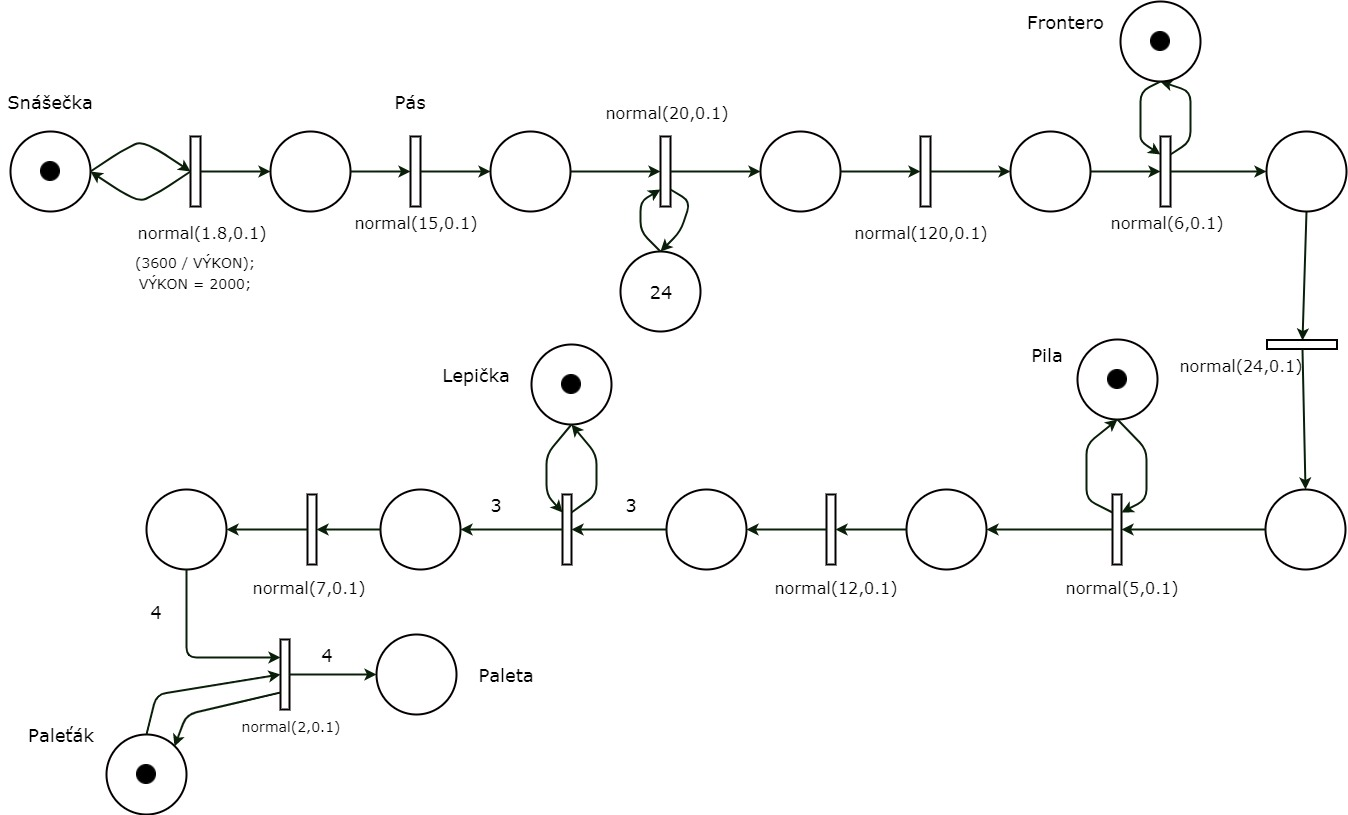
\includegraphics[width=0.95\textwidth]{petri}
	\caption{Petriho síť}
	\label{petri}
\end{figure}

\subsection{Modelování}

Náš model pracuje v real-time čase.

Při měření jsme zjistili, že stroj pracuje jak hodinky, protože všechny naše měření byly téměř stejné. Proto jsme se rozhodli pro normální rozdělení s minimálním rozptylem (\texttt{0.1}) čekání procesů v našem modelu.

\pagebreak

\subsection{Mapování AM na SM}

Jednotlivé přechody mezi mašinami, které jsou viditelné na obrázku \ref{petri}, jsme se rozhodli modelovat jako samostatné procesy.

\begin{itemize}
	\item \textbf{Event::Generator}
	\begin{itemize}
		\item  Tato událost pro nás funguje jako \emph{snášečka}. Generátor se řídí naší konstantou \texttt{SECpBOOK} (doba v sekundách potřebná na jednu knihu), která je vypočítána z~výkonu linky.
	\end{itemize}

	\item \textbf{Process::BlokSL}
	\begin{itemize}
		\item Cesta bloku od snášečka skrz lepičku
	\end{itemize}
	
	\item \textbf{Process::BlokLF}
	\begin{itemize}
		\item Cesta bloku od lepičky skrz frontero
	\end{itemize}
	
	\item \textbf{Process::BlokLP}
	\begin{itemize}
		\item Cesta bloku od lepičky skrz pilu
	\end{itemize}
	
	\item \textbf{Process::BlokLT}
	\begin{itemize}
		\item Cesta bloku od lepičky skrz trojřezu
	\end{itemize}
	
	\item \textbf{Process::BlokFP}
	\begin{itemize}
		\item Cesta bloku od frontera skrz pilu
	\end{itemize}
	
	\item \textbf{Process::BlokFT}
	\begin{itemize}
		\item Cesta bloku od frontera skrz trojřez
	\end{itemize}
	
	\item \textbf{Process::BlokPT}
	\begin{itemize}
		\item Cesta bloku od pily skrz trojřez
	\end{itemize}
	
	\item \textbf{Process::BlokTP}
	\begin{itemize}
		\item Cesta bloku od trojřezu až do paleťáku
	\end{itemize}
	
	\item \textbf{Process::Kniha }
	\begin{itemize}
		\item Kniha na paleťe
	\end{itemize}
	
\end{itemize}

\section{Omezení projektu}

Bohužel se nám nepodařilo implementovat poruchy mašin a jejich opravy. Máme pro toto vytvořenou třídu \texttt{machine\_queue}, která ukládá stav jednotlivých mašin (jede/nejede, poškozena/nepoškozena). Třída je téměř hotova a okomentována, pouze není použita.

Z toho důvodu jsme se zaměřili na výrobu jako takovou bez ohledu na chyby.



\end{document}
